%%---------------------------------------------------------------------------%%
%% compile.tex
%% Time-stamp: <99/02/11 18:42:51 tme>
%% explains how to configure and compile the draco library
%%---------------------------------------------------------------------------%%

\chapter{Configuring and Compiling Draco}
\label{chap:compile}

This chapter describes how to configure and build \draco.  All
configure options will be illuminated in detail.  After reading this
chapter the user and/or developer will know how to build \draco\ on
multiple platforms and for different options.  In addition, the user
will know how to build multiple versions of \draco\ simultaneously.
To illucidate the concepts about \draco\ dependencies, configuration
options, and build targets, \S~\ref{sec:examples} provides several
examples that show how to build \draco\ for various configurations.

%%---------------------------------------------------------------------------%%

\section{Draco Dependencies}
\label{sec:draco_dependencies}

As mentioned in \S~\ref{sec:overview_of_draco}, \draco\ is based on
the concept of levelized design~\cite{la96}.  A package-level diagram
is shown in Fig.~\ref{fig:level}.  By following the dependency lines
\begin{figure}
  \centerline{\includegraphics{fig/level.eps}}
  \caption{Package-level diagram for \draco.}
  \label{fig:level}
\end{figure}
of this diagram, one can determine the exact dependencies required by
each package in \draco.  Thus, to compile a package library, all of
the dependencies, both explicit and implicit, must be included on the
link line.

In addition to the direct package dependencies illustrated in
Fig.~\ref{fig:level}, the \comp{\vble{pkg}/test/} directory may
require additional packages for its conponent tests.  For example,
because most \draco\ packages are templated on Mesh Type, the
component tests for these packages will require a MT.  \draco\ has
several MT packages, \pkg{mesh} and \poomamt, that can be used for
this purpose.  Figure~\ref{fig:test_level} shows the \draco\ package
dependency tree
\begin{figure}
  \centerline{\includegraphics{fig/test_level.eps}}
  \caption{Package-level diagram for \draco.  Test dependencies are
    noted by the dotted arrows.}
  \label{fig:test_level}
\end{figure}
with package test dependencies included. The policy in \draco\ is that
test directories are responsible for their own instantiations.
Directions showing how to include test directory dependencies are
given in Chap~\ref{chap:adding}. 

When using \draco\ on an external product, all package dependent
libraries must be included.  The list of necessary libraries for
linking a package is given in Table~\ref{tab:depends}.  In summary,
\begin{table}
  \caption{
    Listing of \draco\ package dependencies.  The \draco\ Package
    Dependencies are the sum of the Explicit and Implicit Dependencies.
    For general package use, only components listed under \draco\ Package
    Dependencies (Explicit and Implicit) are required.  The components
    listed under \draco\ Package Test Dependencies are only required for
    testing.}
  \label{tab:depends}
  \begin{center}
    \begin{tabular}{lclll} \hline\hline
      \multicolumn{1}{c}{\draco\ Package} & Level &
      \multicolumn{1}{c}{\draco\ Explicit} &
      \multicolumn{1}{c}{\draco\ Implicit} &
      \multicolumn{1}{c}{\draco\ Package} \\ 
      & & \multicolumn{1}{c}{Package Dependencies} &
      \multicolumn{1}{c}{Package Dependencies} &
      \multicolumn{1}{c}{Test Dependencies} \\ \hline
       \dsxx & 1 & - & - & - \\
       \pkg{traits} & 1 & - & - \\ 
       \xm & 1 & - & - & - \\
       \cfour & 2 & \dsxx & - & - \\
       \pkg{nml} & 2 & \dsxx & - & - \\
       \rng & 2 & \dsxx & - & - \\  
       \pkg{units} & 2 & \dsxx & - & - \\
       \pkg{diffusion} & 3 & \pkg{nml} & \dsxx & \pkg{mesh} \\
       \imc & 3 & \dsxx, \rng, \cfour & - & - \\
       \pkg{linalg} & 3 & \dsxx, \cfour, \pkg{nml} & - & - \\
       \pkg{mesh} & 3 & \dsxx, \pkg{xm}, \pkg{traits}, \cfour,
       \pkg{nml} & - & - \\
       \pkg{radphys} & 3 & \pkg{traits}, \pkg{units} & - &
       \pkg{mesh} \\ 
       \pkg{timestep} & 3 & \dsxx, \cfour & - & - \\
       \pkg{matprops} & 4 & \dsxx, \pkg{traits}, \pkg{units},
       \pkg{radphys} & - & \pkg{mesh} \\
       \pone & 4 & \dsxx, \pkg{linalg}, \pkg{diffusion} & \cfour,
       \pkg{nml} & \pkg{mesh} \\ \hline\hline
    \end{tabular}
  \end{center}
\end{table}
when a \draco\ package is used in an external code, all libraries
listed under \draco\ Package Dependencies (Explicit and Implicit) in
Table~\ref{tab:depends} must be included on the link line.  The
packages listed under \draco\ Package Test Dependencies do not have to
be linked.  We note that \draco\ packages know both their package
dependencies (Fig.~\ref{fig:level}) and their package test
dependencies (Fig.~\ref{fig:test_level}).  The external \draco\ client
must be aware that when using a \draco\ package all of the packages
dependencies (not package test dependencies) must be included.

Some components in \draco\ require external vendor support.
Additionally, some configuration options in \draco\ require external
vendor support.  Table~\ref{tab:vendor} lists all of the present
\begin{table}
  \caption{Vendors required by packages in \draco.  Implicit are the
    \cpp\ Standard Template Library (STL), the \cc\ Standard
    Library, and compiler libraries (\comp{libF77}).  Systems
    libraries  (\comp{sys/time.h}) are also not included.}
  \label{tab:vendor}
  \begin{center}
    \begin{tabular}{lclc}\hline\hline
      \multicolumn{1}{c}{Package} & Level & \multicolumn{1}{c}{Vendor Options}
      & Required \\ \hline
      \dsxx & 1 & - &  - \\
      \pkg{traits} & 1 & - & - \\
      \xm & 1 & - & - \\
      \cfour & 2 & \mpi, \shmem & no \\
      \pkg{nml} & 2 & - & - \\
      \rng & 2 & \sprng & yes  \\
      \pkg{units} & 2 & - & - \\
      \pkg{diffusion} & 3 & - & - \\
      \imc & 3 & - & -  \\
      \pkg{linalg} & 3 & \pcglib & yes \\
      \pkg{mesh} & 3 & - & - \\
      \pkg{radphys} & 3 & - & - \\ 
      \pkg{timestep} & 3 & - & - \\
      \pkg{matprops} & 4 & - & - \\
      \pone & 4 & - & - \\ \hline\hline
    \end{tabular}
  \end{center}
\end{table}
packages in \draco\ and the vendors that are required to build those
packages.  Also, because \draco\ is based on the concepts of levelized
design as stated above, each package in \draco\ may have dependencies
on lower level \draco\ packages.  In these cases only the dependencies
of the specified package are of interest.  For example, the \imc\ 
package itself requires no external vendors; however, \imc\ requires
\cfour\ and \rng\ that do require external vendors.  The build system
knows the \draco\ dependencies of each package; however, the external
user (client) must be aware of vendor requirements in the package
dependencies.  Tables~\ref{tab:depends} and \ref{tab:vendor} can be
used to determine what \draco\ packages and what vendor libraries must
be included when linking to a specific \draco\ package.  Details on
how to configure packages with certain vendor options are given in
\S~\ref{sec:configuration_options}.  Information on linking to
specific libraries is given in Appendix~\ref{app:vendor_libs}.

To summarize the preceding we will employ a simple example.  Let us
assume that a user wishes to use the \imc\ package.  Additionally,
this configuration will be a parallel configuration using
\mpi\,\footnote{\cfour\ is \draco's communication package and
  determines if the resulting code will be scalar or parallel.}.  From
Table~\ref{tab:depends} we see that \imc\ is dependent on the \draco\ 
packages \dsxx, \rng, and \cfour.  From Table~\ref{tab:vendor} we see
that \rng\ requires the \sprng\ library and \cfour\ requires the \mpi\ 
library.  Accordingly, the following libraries must be included on the
link line:
\begin{verbatim}
     -limc -lrng -lc4 -lds++ -llfg -lmpi
\end{verbatim}
where \comp{-llfg} is the \sprng\ library, see \S~\ref{appsec:sprng}.
This example assumes that all of the following library locations are
defined in \ldlib.  Thus, even though \imc\ does not explicity depend
on \mpi\ or \sprng, it uses \draco\ packages (\cfour\ and \rng) that
do require these libraries.

%%---------------------------------------------------------------------------%%

\section{Draco Package Products}

In Chap.~\ref{chap:model} we insinuated that each \draco\ package
provides a library.  For example, \imc\ provides
\comp{libimc.a(.so)}.  This is not entifely accurate.  Some \draco\
packages, \xm\ is an example, consist only of header files and do not
provide a compiled library.  Users need to be aware of this fact when
linking \draco\ components.  If a \draco\ client uses the \pkg{mesh}
package, which requires \xm, linking \comp{-lxm} is incorrect because
\xm\ does not produce a library.  Table~\ref{tab:products} lists the
\begin{table}
  \caption{Products for \draco\ packages.}
  \label{tab:products}
  \begin{center}
    \begin{tabular}{lccc}\hline\hline
      \multicolumn{1}{c}{Package} & \comp{include/} & \comp{lib/} &
      \comp{bin/} \\ \hline
      \dsxx & yes & yes & no \\
      \pkg{traits} & yes & no & no \\
      \xm & yes & no & no \\
      \cfour & yes & yes & no \\
      \pkg{nml}$^{\text a}$ & yes & yes & no \\
      \rng & yes & yes & no \\
      \pkg{units} & yes & yes & no \\
      \pkg{diffusion} & yes & yes & no \\
      \imc & yes & yes & no \\
      \pkg{linalg} & yes & yes & no \\
      \pkg{mesh} & yes & yes & no \\
      \pkg{radphys} & yes & yes & no \\
      \pkg{timestep} & yes & yes & no \\
      \pkg{matprops} & yes & yes & no \\
      \pone & yes & yes & no \\
      \hline\hline
      \multicolumn{4}{l}{$^{\text a}$\pkg{nml} uses a \perl\ script
        \comp{nmlgen*} that} \\
      \multicolumn{4}{l}{is installed in the \comp{libexec/}
        directory.} \\
    \end{tabular}    
  \end{center}
\end{table}
\draco\ packages and their products.  Users must only link against
those products that make a library.  Note also that package executables
produced under the \vble{pkg}\comp{/test/} directories are not
considered executable products.

%%---------------------------------------------------------------------------%%

\section{Configuring Draco}
\label{sec:configuring_draco}

We have previously mentioned that building \draco\ is a two-step
process.  First, \draco\ must be configured for a particular build.
Second, \draco\ is built using particular build targets.  In this
section we shall concentrate on configuring \draco.  Note that many
details about configure and \autoconf\ are glossed over in this
treatment.  Interested readers are referred to Ref.~\cite{autoconf}
for more information.  Examples that illustrate the concepts described 
in this section are given in \S~\ref{sec:examples}.

\subsection{Running Configure}
\label{sec:running_configure}

Running configure is straightforward; however, setting up the target
directories where various builds will take place require some
consideration.  In \S~\ref{sec:draco_src_tree} we described how the
source tree is not necessarily where the build takes place.  In fact,
we advise that builds be performed in a location separate from the
source tree.  Through this method multiple builds can be performed
simultaneously.  Additionally, the source tree will not be cluttered
by build-file remnants such as object dependency files.

Before running configure, we set up a target directory tree.  Note
that this directory can be the same as the source directory; although,
we do not recommend this strategy.  The target directory name should
be descriptive of the particular build that is being performed.  For
example to build on a SGI platform with \mpi\ support, one might make
a directory entitled \comp{sgi\_\,mpi/}. Thus, the user enters
\begin{verbatim}
     $ mkdir sgi_mpi
     $ cd sgi_mpi
     $ mkdir draco
\end{verbatim} % $
Note that we do not require a \comp{draco/} directory under the target
directory.  However, this strategy does alleviate the complexity when
using \draco\ with other code systems.  If the user is planning on
using a product that emulates the \draco\ build system, such as
\solon, \tycho, or \milagro, then additional directories should be
added for each product
\begin{verbatim}
     $ cd sgi_mpi
     $ mkdir solon
     $ mkdir tycho
     $ mkdir milagro
\end{verbatim}
Details on using the \draco\ build model in external products are
reserved until Chap.~\ref{chap:extern}.

The next step is to run configure inside the target directory.  We
assume that the \draco\ source tree lives at \dracohome.  We need to
run the configure script, \dracohome\comp{/configure*}, inside of
\comp{sgi\_\,mpi/draco/}.  Most importantly, we need to set the
install directory, denoted by \comp{--prefix} in configure, for
\draco\ components.  This may be accomplished in two ways.  One, the
user may run the \dracoconf\ script that comes with the \draco\ 
distribution.  This script requires the user to set the
\comp{--prefix} directory as an argument to the script. The following
examples illustrate this option:
\begin{verbatim}
     $ cd sgi_mpi/draco
     $ $draco_home/draco_config ..
     $ $draco_home/draco_config .
     $ $draco_home/draco_config /usr/local/contrib/draco
\end{verbatim} % $
The first option sets the install location in \comp{sgi\_\,mpi/}.  The
second option sets the install location in \comp{sgi\_\,mpi/draco/}.
The final option installs in \comp{/usr/local/contrib/draco/}.  The
\dracoconf\ script will give an error if a \comp{--prefix} directory
is not given.  Note that editional options for configure are simply
appended to the command-line.  Thus, to install \draco\ in
\comp{sgi\_\,mpi} with \mpi\ we would enter
\begin{verbatim}
     $ $draco_home/draco_config .. --with-c4=mpi
\end{verbatim}
More details on the configuration options are given in
\S~\ref{sec:configuration_options}.

The second way to run configure is to manually run the
\dracohome\comp{/configure*} script.  Thus, to repeat the options from 
the preceding paragraph, the user must enter
\begin{verbatim}
     $ cd sgi_mpi/draco
     $ $draco_home/configure --prefix=$home/sgi_mpi
     $ $draco_home/configure --prefix=$home/sgi_mpi/draco
     $ $draco_home/configure --prefix=/usr/local/contrib/draco
\end{verbatim} % $
where we have assumed that \comp{sgi\_\,mpi/} lives in \comp{\$home}.
The differences between running \dracoconf\ and
\dracohome\comp{/configure*} should now be apparent.  Configure
expects the directory specified by \comp{--prefix} to be an absolute
path.  \dracoconf\ allows the user to enter relative paths, and it
converts these to absolute paths for configure.  Proceeding with our
analysis, if the user wants to install \draco\ products in
\comp{\$home/sgi\_\,mpi/} with \mpi\ then the following is required
\begin{verbatim}
     $ $draco_home/configure --prefix=$home/sgi_mpi --with-c4=mpi
\end{verbatim} % $
Additional configuration options are detailed in
\S~\ref{sec:configuration_options}. 

Running configure in the \comp{draco/} subdirectory in the target
directory (\comp{sgi\_\,mpi/draco/}) produces a directory tree under
the \comp{draco/} subdirectory that is parallel to the \draco\ source
directory tree.  This directory structure is illustrated in
Fig.~\ref{fig:build_tree}.  Note that we could have run configure
under the target top-level directory (\comp{sgi\_\,mpi/}).  If we had
proceeded with this strategy the contents of the \comp{draco/} target
subdirectory would be moved up one level.

One final point should be mentioned about \comp{--prefix}.  The
default location for the installation directory is
\comp{/usr/local/}.  Thus, the user must enter \comp{--prefix}
explicitly to override the default.  The suggested method is to set
\comp{--prefix} to the target directory (\comp{sgi\_\,mpi/} in this
example).  This will allow multiple targets to be built simultaneously 
without risk of name collisions.

\subsection{Configuration Options}
\label{sec:configuration_options}

Because \draco\ has many packages it must support many configurations.
Additionally, some of these options can be matrixed.  For example,
\draco\ can be configured on SGIs or SPARCs, in 64-bit or 32-bit mode
(SGI only option), scalar or parallel, with shared libraries or
archived libaries, and so forth.  The options that one gives to
configure make clear most of these distinctions. Also, the build
system has built-in intelligence that will try to make the right
choice if incomplete listings for various options are given.

For the standard set of configure options, see Ref.~\cite{autoconf}.
The full set of configure options may be reproduced at the
command-line by entering
\begin{verbatim}
     $ $draco_home/draco_config --help
\end{verbatim}
or 
\begin{verbatim}
     $ $draco_home/configure --help
\end{verbatim}
Note that from this point onward, we will only give examples using
\dracoconf.  As mentioned in the previous section, the built-in
configure variable, \comp{--prefix}, should be set explicitly by the
user to avoid installation of \draco\ components in
\comp{/usr/local/}.

Configuration options come in two forms, \comp{--enable} and
\comp{--with}.  \draco\ policy is to set \comp{--enable} options as
binary switches, whereas \comp{--with} options can take arguments.
Table~\ref{tab:draco-enable} lists the complete set of \comp{--enable}
\begin{table}
  \caption{List of \comp{--enable} options that are unique to \draco.}
  \label{tab:draco-enable}
  \begin{center}
    \begin{tabular}{lcl} \hline\hline
      \multicolumn{1}{c}{Option} & \multicolumn{1}{c}{Default Value} &
      \multicolumn{1}{c}{Description} \\ \hline
                                % --enable-shmem
      \comp{--enable-shmem} & off & turns on \shmem\ communication
      library \\
                                % --enable-pcglib
      \comp{--enable-pcglib} & on & turns off \pcglib \\
                                % --enable-shared
      \comp{--enable-shared} & off & turns on shared (\comp{.so})
      libraries \\
                                % --enable-static-ld
      \comp{--enable-static-ld} & off & tries to use static
      (\comp{.a}) libraries for linking \\
                                % --enable-strict-ansi
      \comp{--enable-strict-ansi} & on & compiles using \comp{strict}
      flags for ANSI compliance \\
                                % --enable-debug
      \comp{--enable-debug} & off & turns on \comp{-g} option for
      debugging$^{\text{a}}$ \\ 
                                % --enable-32-bit
      \comp{--enable-32-bit} & off & turns on 32-bit compiling on SGIs 
      \\ \hline\hline
                                % footnote
      \multicolumn{3}{l}{$^{\text{a}}$the \KCC\ compiler automatically 
        includes \comp{-g} support for optimization level \comp{K0},
        see \S~\ref{sec:optimization}.}
    \end{tabular}
  \end{center}
\end{table}
switches that are unique to \draco.  To turn off a switch the user has
two options, \comp{--enable-switch=no} or \comp{--disable-switch}. The
command-line option \comp{--enable-switch=yes} is equivalent to
\comp{--enable-switch}.  See Ref.~\cite{autoconf} for more details.

The \comp{--with} configure options can take actual arguments.
Table~\ref{tab:draco-with} lists the \comp{--with} options for \draco.
\begin{table}
  \caption{List of \comp{--with} options that are unique to \draco.}
  \label{tab:draco-with}
  \begin{center}
    \begin{tabularx}{\linewidth}{
        >{\setlength{\hsize}{1.1\hsize}}X %
        >{\setlength{\hsize}{1.1\hsize}}X %
        >{\setlength{\hsize}{.6\hsize}}X  %
        >{\setlength{\hsize}{1.1\hsize}}X %
        >{\setlength{\hsize}{1.1\hsize}}X}
      \hline\hline
                                % TABLE HEADINGS
      \multicolumn{1}{c}{Option} & \multicolumn{1}{c}{Valid Arguments} 
      & \multicolumn{1}{c}{Default Value} & \multicolumn{1}{c}{Implied
        Argument} & \multicolumn{1}{c}{Description} \\ \hline\hline
                                % --with-mpi
      \comp{--with-mpi} & \comp{vendor mpich} & \comp{no} &
      \comp{vendor} & see \S~\ref{sec:vendor_libs} \\
                                % --with-mpi-inc
      \comp{--with-mpi-inc} & \vble{dir} & \cnull &
      \comp{\$MPI\_\,INC\_\,DIR} & see \S~\ref{sec:vendor_libs} \\ 
                                % --with-mpi-lib
      \comp{--with-mpi-lib} & \vble{dir} & \cnull &
      \comp{\$MPI\_\,LIB\_\,DIR} & see \S~\ref{sec:vendor_libs} \\
                                % --with-shmem-inc
      \comp{--with-shmem-inc} & \vble{dir} & \cnull &
      \comp{\$SHMEM\_\,INC\_\,DIR} & see \S~\ref{sec:vendor_libs} \\ 
                                % --with-shmem-lib
      \comp{--with-shmem-lib} & \vble{dir} & \cnull &
      \comp{\$SHMEM\_\,LIB\_\,DIR} & see \S~\ref{sec:vendor_libs} \\
                                % --with-sprng
      \comp{--with-sprng} & \comp{lfg lcg} & \comp{lfg} & \comp{lfg} &
      see \S~\ref{sec:vendor_libs} \\
                                % --with-sprng-inc
      \comp{--with-sprng-inc} & \vble{dir} & \cnull & 
      \comp{\$SPRNG\_\,INC\_\,DIR} & see \S~\ref{sec:vendor_libs} \\ 
                                % --with-sprng-lib
      \comp{--with-sprng-lib} & \vble{dir} & \cnull &
      \comp{\$SPRNG\_\,LIB\_\,DIR} & see \S~\ref{sec:vendor_libs} \\
                                % --with-pcglib-lib
      \comp{--with-pcglib-lib} & \vble{dir} & \cnull &
      \comp{\$PCGLIB\_\,LIB\_\,DIR} & see \S~\ref{sec:vendor_libs} \\
                                % --with-c4
      \comp{--with-c4} & \comp{scalar mpi shmem} & \comp{scalar} &
      \comp{scalar} & see \S~\ref{sec:c4_lib} \\
                                % --with-dbc
      \comp{--with-dbc} & \comp{0,1,...,7} & \vble{default} &
      \vble{default} & see \S~\ref{sec:dbc} \\
                                % --with-opt
      \comp{--with-opt} & \comp{0,1,2,3} & \comp{0} & \comp{0} & see
      \S~\ref{sec:optimization} \\
                                % --with-posix
      \comp{--with-posix} & \vble{posix src. num.} & \comp{199309L} &
      \comp{199309L} & sets POSIX source version \\
                                % --with-mips
      \comp{--with-mips} & \comp{1,2,3,4} & \comp{mips4} & \comp{4} &
      sets instruction set on SGIs \\
      \hline\hline
    \end{tabularx}
  \end{center}
\end{table}
Notice that \comp{--with} can be used without arguments.  In this case
an implied argument is assumed by configure.  Thus, \comp{--with}
options have a default value and an implied argument value.  In the
first case, a default value is inferred by configure if the
\comp{--with} option is absent.  In the latter case, an implied
argument is provided if the \comp{--with} option is present but does
not specify an argument.  For example, the following three
configurations are equivalent
\begin{verbatim}
     $ $draco_home/draco_config .. --with-c4=scalar
     $ $draco_home/draco_config .. --with-c4
     $ $draco_home/draco_config .. 
\end{verbatim}
In each case, the \cfour\ package is configured scalar.  In the first
case an explicit argument is given.  In the second case the
\comp{--with-c4} option is given, but the implied argument
(\comp{scalar}) is used.  In the final case the default value for
\comp{--with-c4} is used.  Not all cases have the same defaults for
options and arguments.  An example is the \comp{--with-mpi-inc}
option.  The default is an empty string (\cnull) when the option is
not given.  If the option is given without an argument, configure sets
\comp{--with-mpi-inc=\$MPI\_\,INC\_\,DIR}. In general, the class of
\comp{--with} options that load external libraries work in this
fashion.  Most other \comp{--with} options have the same defaults as
implied arguments.  On a final note, we do not recommend the practice
of setting \comp{--without} because \comp{--with} options are not
meant for binary-type operations.  An exception to this rule is the
vendor-associated options described in \S~\ref{sec:vendor_libs}.

\subsubsection{Vendor Libraries}
\label{sec:vendor_libs}

\draco\ uses external vendors whenever possible to reduce the ammount
of code development required by \draco\ package developers.  The
following vendors are used by \draco:
\begin{itemize}
\item \mpi\ communication library, see \S~\ref{appsec:mpi};
\item \shmem\ communication library, see \S~\ref{appsec:shmem};
\item \sprng\ random number library, see \S~\ref{appsec:sprng};
\item \pcglib\ parallel conjugate gradient solver, see
  \S~\ref{appsec:pcglib}.
\end{itemize}
Vendors are accessed through the \draco\ build system using defined
\comp{--with} and \comp{--enable} tags in \autoconf.
Table~\ref{tab:vendortags} lists the tags from
\begin{table}
  \caption{Tags used to specify vendors in \draco.  See
    Tables~\ref{tab:draco-enable} and \ref{tab:draco-with} for tag
    defaults and implied arguments.}
  \label{tab:vendortags}
  \begin{center}
    \begin{tabular}{la}\hline\hline
      \multicolumn{1}{c}{Vendor} & \multicolumn{1}{c}{\autoconf\ Tags} 
      \\ \hline
                                % MPI
      \mpi & --with-mpi \\
      & --with-mpi-inc \\
      & --with-mpi-lib \\ \hline
                                % SHMEM
      \shmem & --enable-shmem \\
      & --with-shmem-inc \\
      & --with-shmem-lib \\ \hline
                                % SPRNG
      \sprng & --with-sprng \\
      & --with-sprng-inc \\
      & --with-sprng-lib \\ \hline
                                % PCGLIB
      \pcglib & --enable-pcglib \\
      & --with-pcglib-lib \\
      \hline\hline
    \end{tabular}
  \end{center}
\end{table}
Tables~\ref{tab:draco-enable} and \ref{tab:draco-with} that refer
specifically to each vendor used in \draco.  Details on how to use
these tags are given below.

\draco\ vendor libraries are of two types; \latin{required} and
\latin{optional}.  The type classification for each vendor is found in
Table~\ref{tab:vendor}.  \draco\ treats vendors according to the
following rules:
\begin{enumerate}
\item Required vendor libraries are on by default;
\item Optional vendor libraries are off by default.
\end{enumerate}
We note that these rules are applied on a package-by-package basis.
For example, \sprng\ is only required for \rng; thus, \sprng\ is on in
the \rng\ and \imc\ packages (see Table~\ref{tab:depends}).  It is
undefined everywhere else.  This concept applies to all vendor
libraries.

As illustrated in Table~\ref{tab:vendortags}, vendor options are set
by the following three configure tags:
\begin{enumerate}
\item \comp{--with-\vble{vendor}} (\comp{--enable-\vble{vendor}})
  turns the vendor on or off.  If the vendor has options (e.g.
  \comp{--with-mpi}) then \comp{--with} is used.  If the vendor is
  simply on or off (e.g.  \comp{--enable-shmem}) then \comp{--enable}
  is used.
\item \comp{--with-\vble{vendor}-inc} overrides the default \soft{cpp}
  search locations for header files if the vendor is on.
\item \comp{--with-\vble{vendor}-lib} overrides the default search
  path (\ldlib) for libraries if the vendor is on.
\end{enumerate}
Optional vendors may be turned on simply by setting
\comp{--with-\vble{vendor}-inc} or \comp{--with-\vble{vendor}-lib}.
If these tags are set without setting \comp{--with-\vble{vendor}} then
the optional library is turned on, and \comp{--with-\vble{vendor}}
takes the value of its implied argument.  Libraries that use a
\comp{--enable} tag are simply on in this case.  Naturally, the
headers and libraries are searched in the directories given by
\comp{--with-\vble{vendor}-inc} and \comp{--with-\vble{vendor}-lib}.
For required vendors, setting \comp{--with-\vble{vendor}-inc} or
\comp{--with-\vble{vendor}-lib} simply changes the default search
locations for headers and libraries as explained above.

We note that if a required vendor is turned off using
\comp{--without-\vble{vendor}} or \comp{--disable-\vble{vendor}} then
the packages that depend on these vendors will not build.  In other
words, required vendors need not be turned off even if the packages
that use them are not part of a specific \draco\ distribution.
\draco\ knows what packages require what vendors, so turning off
vendors that are not needed in a distribution will have no effect on
the rest of the packages.

\subsubsection{C4 Package Options}
\label{sec:c4_lib}

\cfour\ is \draco's parallel communication package.  It uses either
\mpi\ or \shmem\ to perform message passing operations.  Therefore,
\cfour\ is intimately connected to the \mpi\ and \shmem\ vendors.  The
\autoconf\ tag \comp{--with-c4} determines how \cfour\ should be
configured.  The default option and implied argument is
\comp{--with-c4=scalar}.  However, if \cfour\ is set to \comp{mpi} or
\comp{shmem} then those vendors will be turned on with their implied
argument settings.  Of course, the implied arguments can be overridden
by using the \mpi\ or \shmem\ vendor tags from
Table~\ref{tab:vendortags}.  In summary, if \cfour\ is set to
\comp{mpi} or \comp{shmem}, those libraries will be turned on with all 
default settings.  However, any of the defaults can be changed by
using the \mpi\ and \shmem\ vendor tags that are listed in
Table~\ref{tab:vendortags}. 

\subsubsection{Design-by-Contract}
\label{sec:dbc}

The \comp{--with-dbc} option controls \draco's Design-by-Contract
(DBC) machinery.  DBC support ranges from \comp{0} (lowest) to
\comp{7} (highest).  Table~\ref{tab:dbc} shows the DBC level for
various settings of \comp{--with-dbc}.
\begin{table}
  \caption{DBC support in \draco.}
  \label{tab:dbc}
  \begin{center}
    \begin{tabular}{aa} \hline\hline
      \multicolumn{1}{c}{DBC Setting} & \multicolumn{1}{c}{DBC
        Functions} \\ \hline
      0 &  \\
      1 & Require \\
      2 & Check \\
      3 & Check, Require \\
      4 & Ensure \\
      5 & Ensure, Require \\
      6 & Ensure, Check \\
      7 & Ensure, Check, Require \\ 
      \hline\hline
    \end{tabular}
  \end{center}
\end{table}
If this option is not set (\comp{--with-dbc} is not defined) then the
\dsxx\ package automatically sets DBC to \comp{7}, its highest
setting.  Additionally, the implied argument for \comp{--with-dbc}
sets DBC support to its highest level.  For more information on the
\dsxx\ package DBC and assertion components, see the \dsxx\ manual.

\subsubsection{Optimization}
\label{sec:optimization}

The optimization flags for \KCC, the \cpp\ compiler of choice for
\draco, has some unique options.  Specifically, the lowest level of
optimization, \comp{--with-opt=0}, which is given by default and by
implied argument, automatically sets the \KCC\ compile-line flag,
\comp{+K0}.  The \comp{+K0} option implicitly includes the debug flag
\comp{-g}.  Thus, when \comp{--with-opt=0} the debug flag
(\comp{--enable-debug}) does not have to included.  \draco\ has
built-in intelligence that will turn off the \comp{-g} flag if the
\KCC\ optimization is set to \comp{0}.  The \comp{-g} flag will be
included for any optimization setting greater than \comp{0}.

%%---------------------------------------------------------------------------%%

\section{Building Draco}
\label{sec:building_draco}

After configuration, building \draco\ is mostly straightforward.  In
most cases, one simply enters the target directory, or a target
subdirectory, and runs \gmake.  The \draco\ makefiles include all of
the standard targets listed in The GNU Coding Standard.  For more
detail, see ref.~\cite{gnu}.  Examples of various builds are reserved
until \S~ref{sec:examples}.

\subsection{Building and Installing}

To build and install \draco\ simply enter the
\comp{\vble{target}/draco/} directory and run \comp{gmake}.  At this
level, \gmake\ will enter each subdirectory under
\comp{\vble{target}/draco/} and do a full build followed by an
install.  The default targets in subdirectories under
\comp{\vble{target}/draco/} are different.  Table~\ref{tab:gmake} shows
  the default targets at various
\begin{table}
  \caption{Default targets for \gmake\ at each directory level.  The
    \comp{draco/} directory is a subdirectory of the target directory.}
  \label{tab:gmake}
  \begin{center}
    \begin{tabularx}{\linewidth}{
        >{\setlength{\hsize}{.85\hsize}}L %
        >{\setlength{\hsize}{.75\hsize}}L %
        >{\setlength{\hsize}{1.4\hsize}}X}
      \hline\hline
      \multicolumn{1}{Y}{\draco\ directory} &
      \multicolumn{1}{Y}{Default Target} &
      \multicolumn{1}{Y}{Description} \\ \hline
                                % draco/
      draco/ & install: & builds and installs all sub-directories \\
                                % draco/src
      draco/src & install: & builds and installs all \comp{src/}
      sub-directories \\
                                % draco/src/pkg
      draco/src/\vble{pkg} & lib\vble{pkg}.\vble{suffix}: & builds the
      library for \vble{pkg} \\
                                % draco/src/pkg/test
      draco/src/\vble{pkg}/test & \${test\_\,alltarget}: & builds all of
      the test executables \\
                                % draco/doc
      draco/doc & install dvi: & builds and installs main \draco\
      manual \\
                                % draco/doc/sub-doc
      draco/doc/\vble{sub-doc} & \${manual} & builds the manual
      (\comp{.dvi}) in the \vble{sub-doc/} directory \\
                                % draco/tools
      draco/tools & install: & installs tools into the \comp{libexec}
      directory specified by \comp{--prefix} \\
      \hline\hline
    \end{tabularx}
  \end{center}
\end{table}
levels of the target directory tree.  If \gmake\ is run at levels
lower than the \comp{\vble{target}/draco/src/} directory, the user
must be aware of package dependencies.  For example, \cfour\ cannot be
built if \dsxx\ has not been built and installed.  Thus, the general
user should avoid manual builds of packages at the
\comp{\vble{target}/draco/src/\vble{pkg}/} level.  At higher levels,
\draco\ knows how to build packages in the proper order.

At each target directory level the \draco\ build system knows nothing
about dependency packages at the same level except that they do or do
not exist.  Thus, \cfour\ simply checks to see if \dsxx\ has been
installed.  If \dsxx\ does not exist in the install location specified
by \comp{--prefix} then \gmake\ will end.  This aspect of the build
system is a feature for \draco\ developers.  It gives developers the
flexibility to modify code in a package and test it without affecting
other packages that may depend on that code.  One drawback is that
users must be aware of the package dependencies when performing manual
builds.  These dependencies are illustrated in Fig.~\ref{fig:level}
and are listed in Table~\ref{tab:depends}.

The \comp{check} target runs the component tests in each package
directory before installation.  This is done to conform to the GNU
Standard, which states that tests should not be dependent upon
installation.  The \comp{check} target uses \dejagnu\ to generate test 
output data and results.  For more information, see
ref.~\cite{dejagnu}.  A future \draco\ document will describe the
details of \draco\ regression testing.

An additional feature of the \draco\ build system is that \draco\ will 
automatically run \autoconf\ if any of the configure system files have 
been adapted.  Thus, if \comp{aclocal.m4} or \comp{Makefile.in} are
changed then \gmake\ will reconfigure the affected directories.  

\subsection{Build Targets}

A detailed discussion of all the build targets in the GNU Coding
Standard is beyond the scope of this text. For more information the
reader is advised to study ref.~\cite{gnu}.  What follows is a brief
description of the makefile targets in \draco\ and what operations
they perform.
\begin{description}
\item[\comp{install}]\index{gmake!target!install|textbf} \gmake\ will
  build all subdirectories that exist at the current level; it will
  then install the products in the locations specified by
  \comp{--prefix}.  In each subdirectory, build products are installed
  before moving on to the next directory.
\item[\comp{check}]\index{gmake!target!check|textbf} \gmake\ will
  build all subdirectories that exist at the current level; it will
  then run the \comp{test/} directory components using \dejagnu.  If
  this target is run from the \comp{draco/} or \comp{draco/src} level
  then installation will follow the test runs.
\item[\comp{install dvi}]\index{gmake!target!install dvi|textbf}
  \gmake\ will build and install the main \draco\ manual when this is
  run from the \comp{draco/} or \comp{draco/doc/} directories.  When
  this target is run from a \comp{draco/doc/\vble{sub-doc}/} directory
  it will build the \vble{sub-doc} manual and install it.
\item[\comp{dvi}]\index{gmake!target!dvi|textbf} \gmake\ will build
  the manual in the directory where this target is run.  In
  \comp{draco/doc/} it will build the main manual.  In
  \comp{draco/doc/\vble{sub-doc}/} it will build the \vble{sub-doc}
  manual.
\item[\comp{clean}]\index{gmake!target!clean|textbf} \gmake\ will
  clean the compiled files (\comp{*.d} and \comp{*.o}) from the target
  sub-directories.
\item[randy] Randy must write much more here.
\end{description}
These targets have been designed to satisfy the needs of users, who
perform one-time global builds, and developers, who perform multiple
local builds.

%%---------------------------------------------------------------------------%%

\section{Recommended Practices}

Although \draco\ can be configured and built in any number of ways, we 
have a set of ``standard'' recommended practices that are followed by
\draco\ team members.  This methodology for configuring and
building \draco\ is summarized in the following steps:
\begin{enumerate}
\item Checkout a version of \draco; the location of which is
  \dracohome.
\item Make a target directory that appropriately describes the
  configuration options; we call this directory \comp{\vble{target}/}.
\item Make a \comp{draco/} subdirectory under the target directory,
  ie. \comp{\vble{target}/draco/}.
\item Run \dracohome\comp{/draco\_\,config*} in
  \comp{\vble{target}/draco/} with the appropriate options for this
  configuration.  Set \comp{--prefix=\vble{target}/}. Thus, the
  configure line is:
  \begin{alltt}
    $ $draco_home/draco_config .. \vble{options}
  \end{alltt}
\item Run \gmake\ in \comp{\vble{target}/draco/};
\begin{verbatim}
    $ gmake
\end{verbatim} % $
  This step will build and install all of the \draco\ products from
  each subdirectory under \comp{\vble{target}/draco/}.  The headers
  will be installed in \comp{\vble{target}/include/}.  The libraries
  will be installed in \comp{\vble{target}/lib/}. And, the
  package-dependent executables will be installed in
  \comp{\vble{target}/libexec}.
\end{enumerate}
This procedure simplifies adding an external code system that uses,
and is based on, \draco.  For example, \solon\ uses \draco\ as a
build-model template.  Thus, we can add a \comp{\vble{target}/solon}
directory and configure, build, and install \solon\ in the same
location as \draco\ products.  Details on this process are given in
\S~\ref{sec:emulating}. 

%%---------------------------------------------------------------------------%%

\section{Examples}
\label{sec:examples}

To illucidate some of the concepts that we have described in this
chapter, we proceed to show some configuration and build examples.
The following examples give a cross section of the processes that
\draco\ users and developers will use.
\begin{cexa}
  \label{ex:basic}
  Build a scalar version of \draco.  \sprng\ headers are in the
  \soft{cpp} include path, and \sprng\ and \pcglib\ libraries are
  found in \ldlib.  The \draco\ source directory is
  \comp{/usr/tmp/joe/draco}.  We want \draco\ installed in
  \comp{/usr/local/draco}.
\end{cexa}
\begin{proof}[Solution to \ref{ex:basic}]
  First, we need to make a target directory.  In
  \S~\ref{sec:running_configure} we advised not to use the source
  directory as the build directory.  We will follow this policy and
  make our target directory \comp{draco\_\,target}:
\begin{verbatim}
     $ cd /usr/local/draco
     $ mkdir draco_target
\end{verbatim}
  Note that we could have called \comp{draco\_\,target/}
  \comp{draco/}.  We used a different name to illustrate the
  independence of the target-build directory.  Now, we configure
  \draco\ according to the specification in Ex.~\ref{ex:basic}.  This
  configuration is scalar so we can use the default setting for
  \cfour.  Additionally, all of the required vendors are located in
  default locations.
\begin{verbatim}
     $ cd draco_target
     $ /usr/tmp/joe/draco/draco_config ..
\end{verbatim}
  \dracoconf\ expands the relative path argument, \comp{..}, into
  \comp{--prefix=/usr/local/draco}.  All other defaults are used.
  Finally, we want to do a build and install of all \draco\ products;
  thus, according to \S~\ref{sec:building_draco}, we must enter
\begin{verbatim}
     $ gmake
\end{verbatim} % $
  We also could have entered \comp{gmake install}; however,
  Table~\ref{tab:gmake} shows that the default target at the highest
  level is \comp{install}.
\end{proof}

Example~\ref{ex:basic} is straightforward.  We will now give a series
of examples and solutions that involve more detailed configurations
and builds.  At this point, we will only show the steps in the
solution procedure.  The details about each step can be inferred from
\S~\ref{sec:configuring_draco} and \ref{sec:building_draco}.

\begin{cexa}
  \label{ex:mpi}
  Build a version of \draco\ with \mpi.  Additionally, this build
  takes place on an SGI with \comp{\$MPT\_\,SGI} loaded as a module.
  Thus, we are using the SGI vendor version of \mpi.  \sprng\ is
  located in \comp{/usr/local/sprng} and \pcglib\ is in the \ldlib.
\end{cexa}
\begin{proof}[Solution to \ref{ex:mpi}]
  Before proceeding to the solution, we note that the \draco\ build
  system knows about the SGI Message Passing Toolkit (MPT) module.
  Thus, setting the include and library paths for \mpi\ is not
  required.
\begin{verbatim}
     $ cd /usr/local/draco
     $ mkdir draco
     $ cd draco
     $ /usr/tmp/joe/draco/draco_config .. --with-c4=mpi --with-sprng-inc=
     /usr/local/sprng/SRC --with-sprng-lib=/usr/local/sprng/lib
     $ gmake
\end{verbatim} % $
\end{proof}

\begin{cexa}
  \label{ex:mpich}
  Build a version of \draco\ with \mpi\ and optimization set to level
  \comp{3}.  Turn off all DBC support.  Use the \sys{mpich} version of
  \mpi\ that is installed in \comp{/usr/local/}. \pcglib\ is in
  \comp{/usr/local/pcg}.  This could be considered a production
  version of \draco.
\end{cexa}
\begin{proof}[Solution to \ref{ex:mpich}]
  We will proceed in a slightly different manner than the previous
  examples.  Here we will use environment variables to determine the
  location of \sprng.  We assume the \soft{BASH} shell is in use.
\begin{verbatim}
     $ export SPRNG_INC_DIR=/usr/local/sprng/SRC
     $ export SPRNG_LIB_DIR=/usr/local/sprng/lib
     $ cd /usr/local/draco
     $ mkdir draco
     $ cd draco
     $ /usr/tmp/joe/draco/draco_config .. --with-c4=mpi --with-sprng-inc
     --with-sprng-lib --with-pcglib-lib=/usr/local/pcg/lib --with-mpi=mpich
     --with-mpi-inc=/usr/local/include --with-mpi-lib=/usr/local/lib 
     --with-opt=3 --with-dbc=0
\end{verbatim}
\end{proof}

%%---------------------------------------------------------------------------%%

\section{Summary}

We have given a tutorial on how to configure and build \draco.  The
package and vendor dependencies in \draco\ have been listed in
\S~\ref{sec:draco_dependencies}.  Details on configuring and
building \draco\ have been given in \S~\ref{sec:configuring_draco} and 
\ref{sec:building_draco}.  We have tied these concepts together with
several examples in \S~\ref{sec:examples}.
